% Options for packages loaded elsewhere
\PassOptionsToPackage{unicode}{hyperref}
\PassOptionsToPackage{hyphens}{url}
%
\documentclass[
  10pt,
]{article}
\usepackage{amsmath,amssymb}
\usepackage{lmodern}
\usepackage{ifxetex,ifluatex}
\ifnum 0\ifxetex 1\fi\ifluatex 1\fi=0 % if pdftex
  \usepackage[T1]{fontenc}
  \usepackage[utf8]{inputenc}
  \usepackage{textcomp} % provide euro and other symbols
\else % if luatex or xetex
  \usepackage{unicode-math}
  \defaultfontfeatures{Scale=MatchLowercase}
  \defaultfontfeatures[\rmfamily]{Ligatures=TeX,Scale=1}
\fi
% Use upquote if available, for straight quotes in verbatim environments
\IfFileExists{upquote.sty}{\usepackage{upquote}}{}
\IfFileExists{microtype.sty}{% use microtype if available
  \usepackage[]{microtype}
  \UseMicrotypeSet[protrusion]{basicmath} % disable protrusion for tt fonts
}{}
\makeatletter
\@ifundefined{KOMAClassName}{% if non-KOMA class
  \IfFileExists{parskip.sty}{%
    \usepackage{parskip}
  }{% else
    \setlength{\parindent}{0pt}
    \setlength{\parskip}{6pt plus 2pt minus 1pt}}
}{% if KOMA class
  \KOMAoptions{parskip=half}}
\makeatother
\usepackage{xcolor}
\IfFileExists{xurl.sty}{\usepackage{xurl}}{} % add URL line breaks if available
\IfFileExists{bookmark.sty}{\usepackage{bookmark}}{\usepackage{hyperref}}
\hypersetup{
  pdftitle={Summary Report COVID Contact Tracing Côte d'Ivoire},
  hidelinks,
  pdfcreator={LaTeX via pandoc}}
\urlstyle{same} % disable monospaced font for URLs
\usepackage[margin=1in]{geometry}
\usepackage{graphicx}
\makeatletter
\def\maxwidth{\ifdim\Gin@nat@width>\linewidth\linewidth\else\Gin@nat@width\fi}
\def\maxheight{\ifdim\Gin@nat@height>\textheight\textheight\else\Gin@nat@height\fi}
\makeatother
% Scale images if necessary, so that they will not overflow the page
% margins by default, and it is still possible to overwrite the defaults
% using explicit options in \includegraphics[width, height, ...]{}
\setkeys{Gin}{width=\maxwidth,height=\maxheight,keepaspectratio}
% Set default figure placement to htbp
\makeatletter
\def\fps@figure{htbp}
\makeatother
\setlength{\emergencystretch}{3em} % prevent overfull lines
\providecommand{\tightlist}{%
  \setlength{\itemsep}{0pt}\setlength{\parskip}{0pt}}
\setcounter{secnumdepth}{5}
% \usepackage[export]{adjustbox}
\usepackage{fancyhdr}
\pagestyle{fancy}
% \usepackage{framed}
% \usepackage{tcolorbox}
% \usepackage{tikz}
% \usetikzlibrary{calc}
% \usepackage{tikzpagenodes}
\usepackage{float}
% \usepackage{booktabs}
% \usepackage{tabularx}
% \usepackage{colortbl}
% \usepackage{graphicx}
% \usepackage{longtable}

%sans-serif font
% \usepackage{helvet}
% \renewcommand{\familydefault}{\sfdefault} % sans serif
% \fontfamily{ppl}\selectfont
% 
% \makeatletter
% \global\let\tikz@ensure@dollar@catcode=\relax
% \makeatother

\fancyhf{}

% \chead{
% \vspace{2cm}
% 
\includegraphics[width=21.7cm,height = 7cm, center]{who_header.png}
% }

% numbering pages
\fancyfoot[C]{

\includegraphics[width=21.7cm,height = 4cm, center]{who_footer.png}
}

% \def\chpcolor{blue!60!green}
% \def\chpcolortxt{blue!60!green}
% \def\sectionfont{\sffamily\LARGE}
% 
% \setcounter{secnumdepth}{2}
% 
% \makeatletter
% %Section:
% \def\@sectionstrut{\vrule\@width\z@\@height12.5\p@}
% \def\@makesectionhead#1{%
%   {\par\vspace{20pt}%
%    \parindent 0pt\raggedleft\sectionfont
%    \colorbox{\chpcolor}{%
%      \parbox[t]{90pt}{\color{white}\@sectionstrut\@depth4.5\p@\hfill
%        \ifnum\c@secnumdepth>\z@\thesection\fi}%
%    }%
%    \begin{minipage}[t]{\dimexpr\textwidth-90pt-2\fboxsep\relax}
%    \color{\chpcolortxt}\@sectionstrut\hspace{5pt}#1
%    \end{minipage}\par
%    \vspace{10pt}%
%   }
% }
% \def\section{\@afterindentfalse\secdef\@section\@section}
% \def\@section[#1]#2{%
%   \ifnum\c@secnumdepth>\m@ne
%     \refstepcounter{section}%
%     \addcontentsline{toc}{section}{\protect\numberline{\thesection}#1}%
%   \else
%     \phantomsection
%     \addcontentsline{toc}{section}{#1}%
%   \fi
%   \sectionmark{#1}%
%   \if@twocolumn
%     \@topnewpage[\@makesectionhead{#2}]%
%   \else
%     \@makesectionhead{#2}\@afterheading
%   \fi
% }
\usepackage{array}
\usepackage{caption}
\usepackage{graphicx}
\usepackage{siunitx}
\usepackage[normalem]{ulem}
\usepackage{colortbl}
\usepackage{multirow}
\usepackage{hhline}
\usepackage{calc}
\usepackage{tabularx}
\usepackage{threeparttable}
\usepackage{wrapfig}
\usepackage{adjustbox}
\usepackage{hyperref}
\ifluatex
  \usepackage{selnolig}  % disable illegal ligatures
\fi

\title{Summary Report COVID Contact Tracing Côte d'Ivoire}
\author{}
\date{\vspace{-2.5em}}

\begin{document}
\maketitle

{
\setcounter{tocdepth}{2}
\tableofcontents
}
\chead{
\Huge
\textbf{CovContactR Report}\\
\Large
Cotê d'Ivoire \\
From 2021-01-04 to 2021-04-22
}

\hypertarget{value-box-summaries}{%
\subsection{Value box summaries}\label{value-box-summaries}}

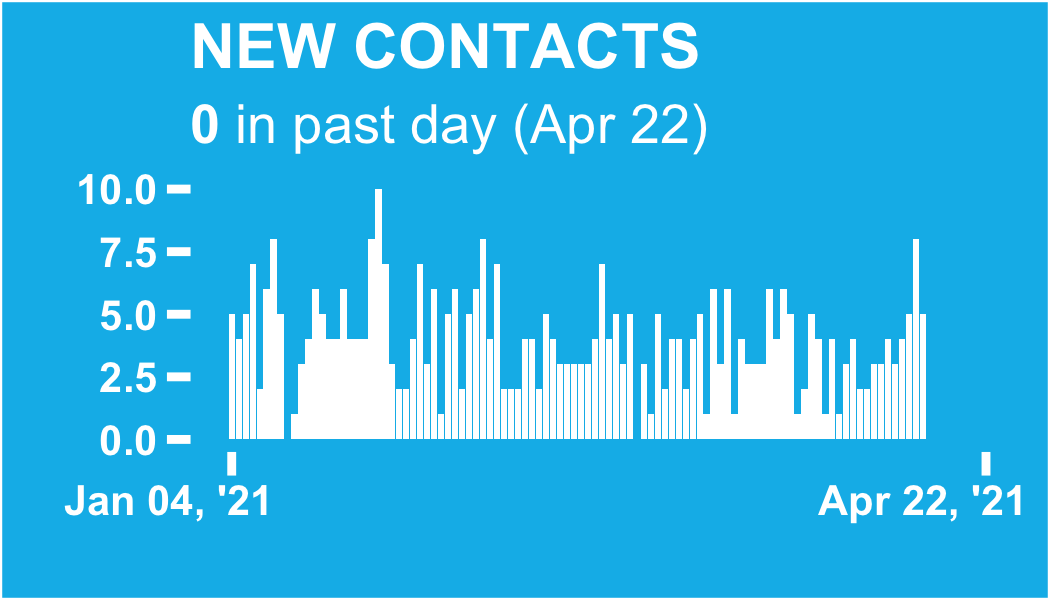
\includegraphics[width=0.48\linewidth]{report_files/figure-latex/unnamed-chunk-5-1}
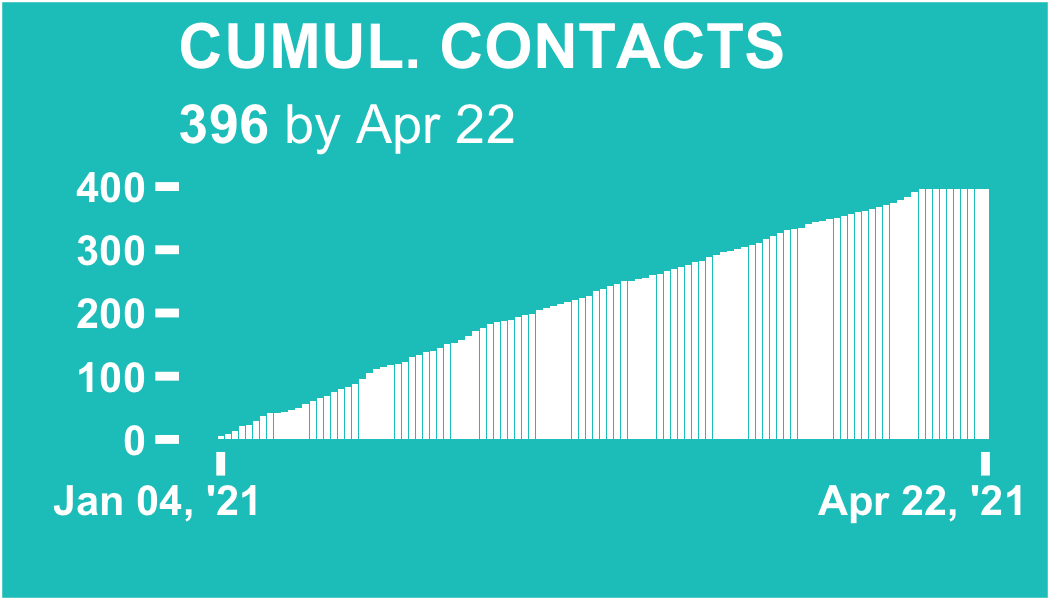
\includegraphics[width=0.48\linewidth]{report_files/figure-latex/unnamed-chunk-5-2}

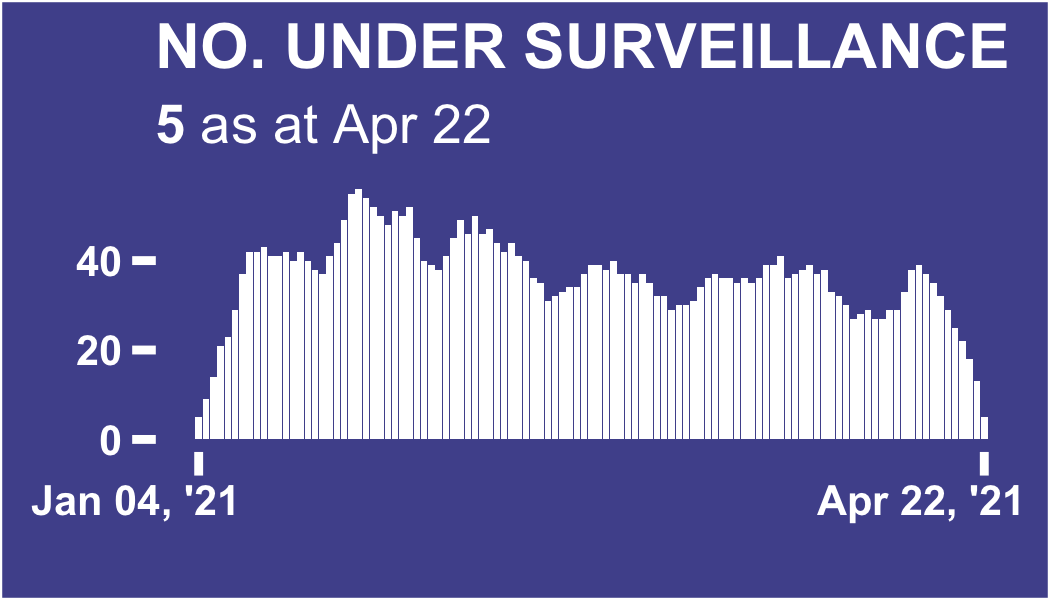
\includegraphics[width=0.48\linewidth]{report_files/figure-latex/unnamed-chunk-6-1}
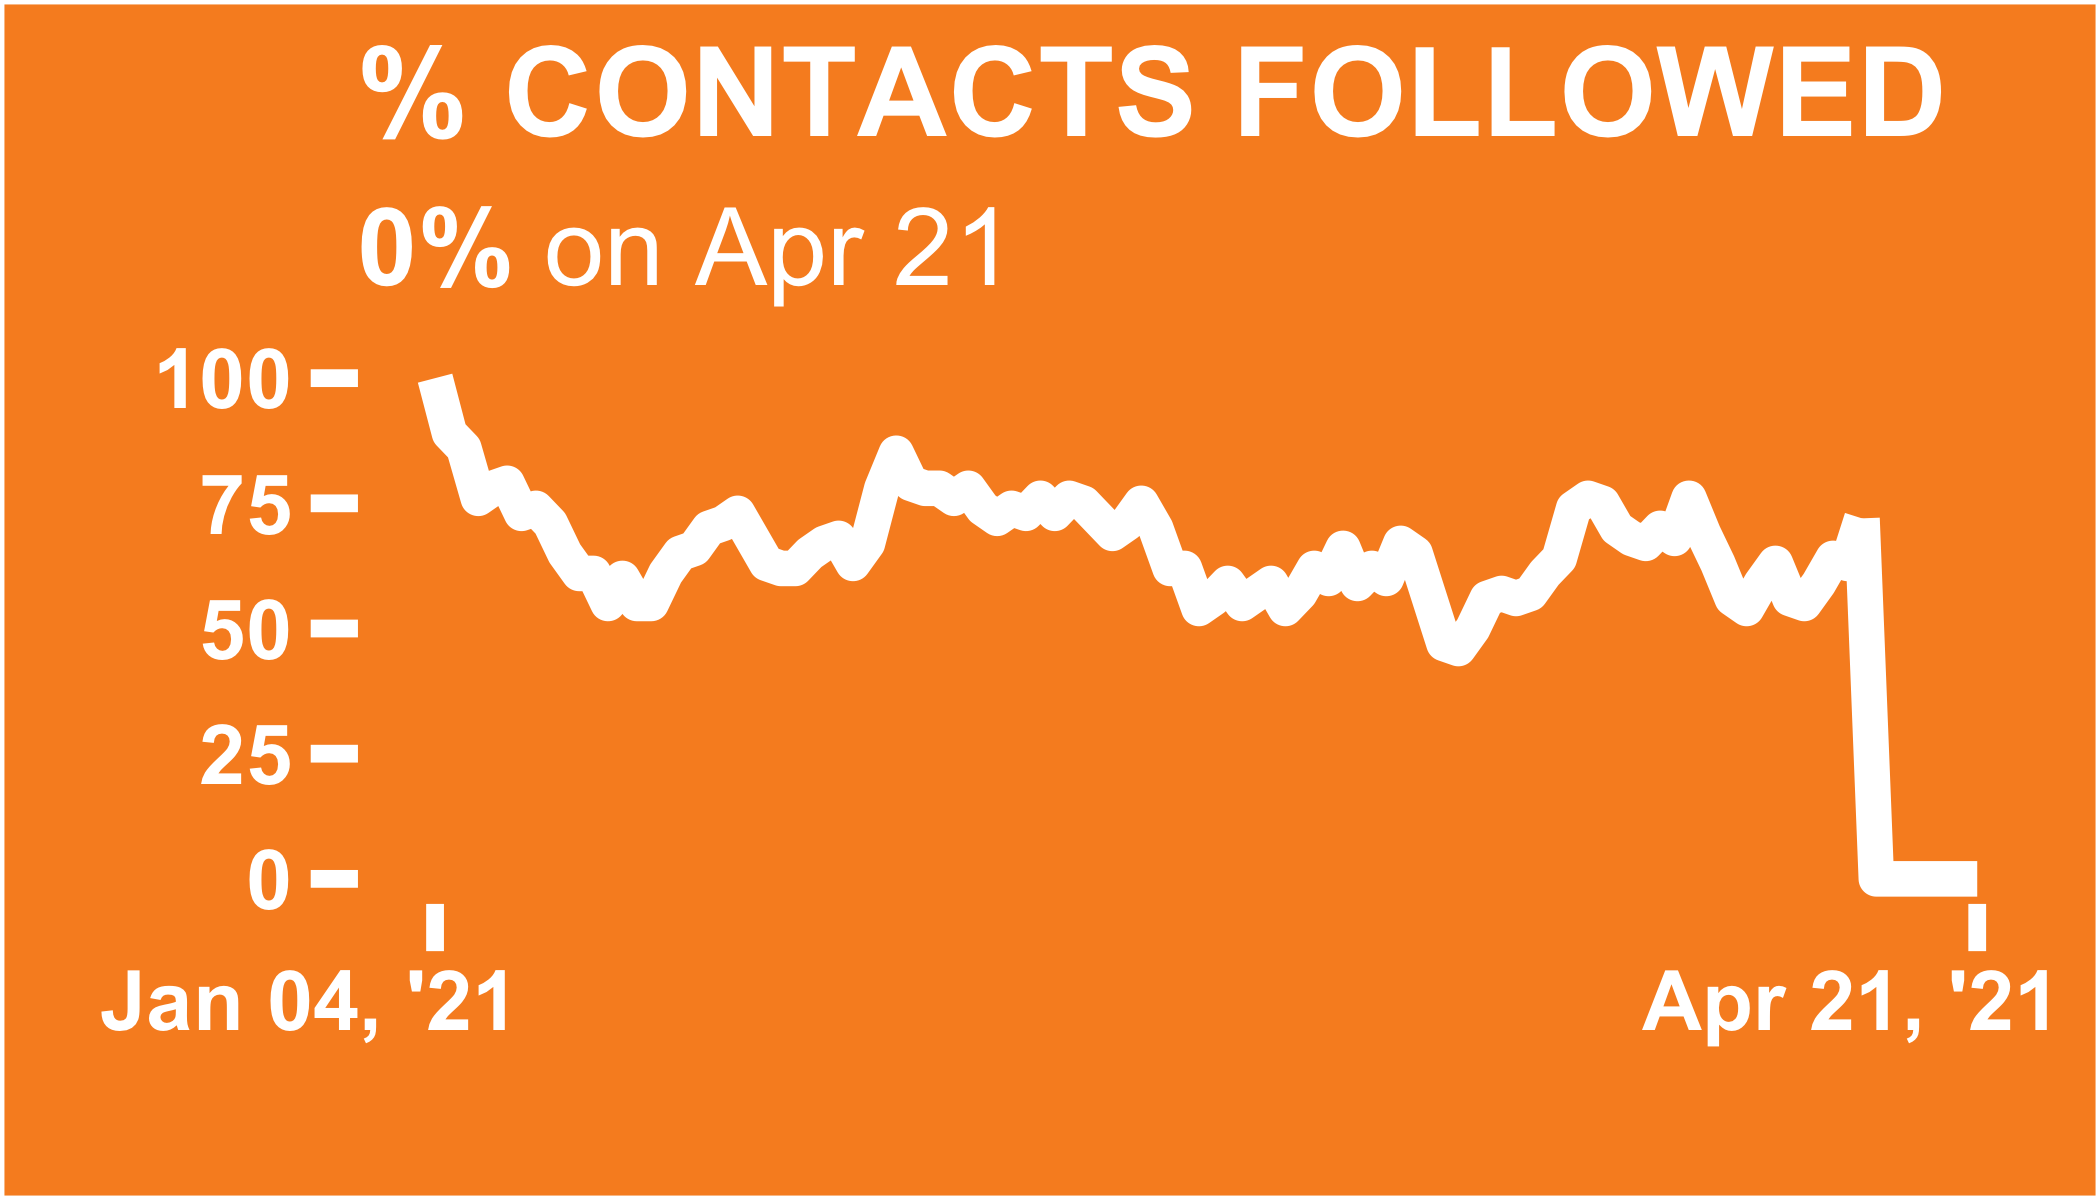
\includegraphics[width=0.48\linewidth]{report_files/figure-latex/unnamed-chunk-6-2}

\hypertarget{all-contacts}{%
\section{All contacts}\label{all-contacts}}

\hypertarget{total-contacts-per-region}{%
\subsection{Total contacts per region}\label{total-contacts-per-region}}

ℹ: The table and plot show the count of all contacts recorded in each
region since database inception.

The region with the most total contacts since database inception is
Abidjan 2, with 193 contacts (48.7\% of the total)

\hypertarget{table}{%
\subsection{Table}\label{table}}

 
  \providecommand{\huxb}[2]{\arrayrulecolor[RGB]{#1}\global\arrayrulewidth=#2pt}
  \providecommand{\huxvb}[2]{\color[RGB]{#1}\vrule width #2pt}
  \providecommand{\huxtpad}[1]{\rule{0pt}{#1}}
  \providecommand{\huxbpad}[1]{\rule[-#1]{0pt}{#1}}

\begin{table}[h!]
\begin{centerbox}
\begin{threeparttable}
 \label{tab:unnamed-chunk-8}
\setlength{\tabcolsep}{0pt}
\begin{tabular}{l l l l}


\hhline{>{\huxb{255, 255, 255}{1}}->{\huxb{255, 255, 255}{1}}->{\huxb{255, 255, 255}{1}}->{\huxb{255, 255, 255}{1}}-}
\arrayrulecolor{black}

\multicolumn{1}{!{\huxvb{255, 255, 255}{1}}l!{\huxvb{255, 255, 255}{1}}}{\cellcolor[RGB]{84, 153, 199}\huxtpad{0.5pt + 1em}\raggedright \hspace{6pt} \textbf{\textcolor[RGB]{255, 255, 255}{Region}} \hspace{0.5pt}\huxbpad{0.5pt}} &
\multicolumn{1}{l!{\huxvb{255, 255, 255}{1}}}{\cellcolor[RGB]{84, 153, 199}\huxtpad{0.5pt + 1em}\raggedright \hspace{0.5pt} \textbf{\textcolor[RGB]{255, 255, 255}{District}} \hspace{0.5pt}\huxbpad{0.5pt}} &
\multicolumn{1}{r!{\huxvb{255, 255, 255}{1}}}{\cellcolor[RGB]{84, 153, 199}\huxtpad{0.5pt + 1em}\raggedleft \hspace{0.5pt} \textbf{\textcolor[RGB]{255, 255, 255}{Total contacts}} \hspace{0.5pt}\huxbpad{0.5pt}} &
\multicolumn{1}{r!{\huxvb{255, 255, 255}{1}}}{\cellcolor[RGB]{84, 153, 199}\huxtpad{0.5pt + 1em}\raggedleft \hspace{0.5pt} \textbf{\textcolor[RGB]{255, 255, 255}{\%}} \hspace{6pt}\huxbpad{0.5pt}} \tabularnewline[-0.5pt]


\hhline{>{\huxb{255, 255, 255}{1}}->{\huxb{255, 255, 255}{1}}->{\huxb{255, 255, 255}{1}}->{\huxb{255, 255, 255}{1}}-}
\arrayrulecolor{black}

\multicolumn{1}{!{\huxvb{255, 255, 255}{1}}l!{\huxvb{255, 255, 255}{1}}}{\cellcolor[RGB]{212, 230, 241}} &
\multicolumn{1}{l!{\huxvb{255, 255, 255}{1}}}{\cellcolor[RGB]{212, 230, 241}\huxtpad{0.5pt + 1em}\raggedright \hspace{0.5pt} Adjame \& plateau \& attecoube \hspace{0.5pt}\huxbpad{0.5pt}} &
\multicolumn{1}{r!{\huxvb{255, 255, 255}{1}}}{\cellcolor[RGB]{212, 230, 241}\huxtpad{0.5pt + 1em}\raggedleft \hspace{0.5pt} 50 \hspace{0.5pt}\huxbpad{0.5pt}} &
\multicolumn{1}{r!{\huxvb{255, 255, 255}{1}}}{\cellcolor[RGB]{212, 230, 241}\huxtpad{0.5pt + 1em}\raggedleft \hspace{0.5pt} 12.6~ \hspace{6pt}\huxbpad{0.5pt}} \tabularnewline[-0.5pt]


\hhline{>{\huxb{255, 255, 255}{1}}|>{\huxb{212, 230, 241}{1}}->{\huxb{255, 255, 255}{1}}|>{\huxb{255, 255, 255}{1}}->{\huxb{255, 255, 255}{1}}->{\huxb{255, 255, 255}{1}}-}
\arrayrulecolor{black}

\multicolumn{1}{!{\huxvb{255, 255, 255}{1}}l!{\huxvb{255, 255, 255}{1}}}{\cellcolor[RGB]{212, 230, 241}} &
\multicolumn{1}{l!{\huxvb{255, 255, 255}{1}}}{\cellcolor[RGB]{169, 204, 227}\huxtpad{0.5pt + 1em}\raggedright \hspace{0.5pt} Port bouet \& vridi \hspace{0.5pt}\huxbpad{0.5pt}} &
\multicolumn{1}{r!{\huxvb{255, 255, 255}{1}}}{\cellcolor[RGB]{169, 204, 227}\huxtpad{0.5pt + 1em}\raggedleft \hspace{0.5pt} 41 \hspace{0.5pt}\huxbpad{0.5pt}} &
\multicolumn{1}{r!{\huxvb{255, 255, 255}{1}}}{\cellcolor[RGB]{169, 204, 227}\huxtpad{0.5pt + 1em}\raggedleft \hspace{0.5pt} 10.3~ \hspace{6pt}\huxbpad{0.5pt}} \tabularnewline[-0.5pt]


\hhline{>{\huxb{255, 255, 255}{1}}|>{\huxb{212, 230, 241}{1}}->{\huxb{255, 255, 255}{1}}|>{\huxb{255, 255, 255}{1}}->{\huxb{255, 255, 255}{1}}->{\huxb{255, 255, 255}{1}}-}
\arrayrulecolor{black}

\multicolumn{1}{!{\huxvb{255, 255, 255}{1}}l!{\huxvb{255, 255, 255}{1}}}{\cellcolor[RGB]{212, 230, 241}} &
\multicolumn{1}{l!{\huxvb{255, 255, 255}{1}}}{\cellcolor[RGB]{212, 230, 241}\huxtpad{0.5pt + 1em}\raggedright \hspace{0.5pt} Cocody bingerville \hspace{0.5pt}\huxbpad{0.5pt}} &
\multicolumn{1}{r!{\huxvb{255, 255, 255}{1}}}{\cellcolor[RGB]{212, 230, 241}\huxtpad{0.5pt + 1em}\raggedleft \hspace{0.5pt} 40 \hspace{0.5pt}\huxbpad{0.5pt}} &
\multicolumn{1}{r!{\huxvb{255, 255, 255}{1}}}{\cellcolor[RGB]{212, 230, 241}\huxtpad{0.5pt + 1em}\raggedleft \hspace{0.5pt} 10.1~ \hspace{6pt}\huxbpad{0.5pt}} \tabularnewline[-0.5pt]


\hhline{>{\huxb{255, 255, 255}{1}}|>{\huxb{212, 230, 241}{1}}->{\huxb{255, 255, 255}{1}}|>{\huxb{255, 255, 255}{1}}->{\huxb{255, 255, 255}{1}}->{\huxb{255, 255, 255}{1}}-}
\arrayrulecolor{black}

\multicolumn{1}{!{\huxvb{255, 255, 255}{1}}l!{\huxvb{255, 255, 255}{1}}}{\cellcolor[RGB]{212, 230, 241}} &
\multicolumn{1}{l!{\huxvb{255, 255, 255}{1}}}{\cellcolor[RGB]{169, 204, 227}\huxtpad{0.5pt + 1em}\raggedright \hspace{0.5pt} Koumassi \hspace{0.5pt}\huxbpad{0.5pt}} &
\multicolumn{1}{r!{\huxvb{255, 255, 255}{1}}}{\cellcolor[RGB]{169, 204, 227}\huxtpad{0.5pt + 1em}\raggedleft \hspace{0.5pt} 33 \hspace{0.5pt}\huxbpad{0.5pt}} &
\multicolumn{1}{r!{\huxvb{255, 255, 255}{1}}}{\cellcolor[RGB]{169, 204, 227}\huxtpad{0.5pt + 1em}\raggedleft \hspace{0.5pt} 8.33 \hspace{6pt}\huxbpad{0.5pt}} \tabularnewline[-0.5pt]


\hhline{>{\huxb{255, 255, 255}{1}}|>{\huxb{212, 230, 241}{1}}->{\huxb{255, 255, 255}{1}}|>{\huxb{255, 255, 255}{1}}->{\huxb{255, 255, 255}{1}}->{\huxb{255, 255, 255}{1}}-}
\arrayrulecolor{black}

\multicolumn{1}{!{\huxvb{255, 255, 255}{1}}l!{\huxvb{255, 255, 255}{1}}}{\multirow[t]{-5}{*}[0ex]{\cellcolor[RGB]{212, 230, 241}\huxtpad{0.5pt + 1em}\raggedright \hspace{6pt} Abidjan 2 \hspace{0.5pt}\huxbpad{0.5pt}}} &
\multicolumn{1}{l!{\huxvb{255, 255, 255}{1}}}{\cellcolor[RGB]{212, 230, 241}\huxtpad{0.5pt + 1em}\raggedright \hspace{0.5pt} Trechville \& marcory \hspace{0.5pt}\huxbpad{0.5pt}} &
\multicolumn{1}{r!{\huxvb{255, 255, 255}{1}}}{\cellcolor[RGB]{212, 230, 241}\huxtpad{0.5pt + 1em}\raggedleft \hspace{0.5pt} 29 \hspace{0.5pt}\huxbpad{0.5pt}} &
\multicolumn{1}{r!{\huxvb{255, 255, 255}{1}}}{\cellcolor[RGB]{212, 230, 241}\huxtpad{0.5pt + 1em}\raggedleft \hspace{0.5pt} 7.32 \hspace{6pt}\huxbpad{0.5pt}} \tabularnewline[-0.5pt]


\hhline{>{\huxb{255, 255, 255}{1}}->{\huxb{255, 255, 255}{1}}->{\huxb{255, 255, 255}{1}}->{\huxb{255, 255, 255}{1}}-}
\arrayrulecolor{black}

\multicolumn{1}{!{\huxvb{255, 255, 255}{1}}l!{\huxvb{255, 255, 255}{1}}}{\cellcolor[RGB]{169, 204, 227}} &
\multicolumn{1}{l!{\huxvb{255, 255, 255}{1}}}{\cellcolor[RGB]{169, 204, 227}\huxtpad{0.5pt + 1em}\raggedright \hspace{0.5pt} Yopougan est \hspace{0.5pt}\huxbpad{0.5pt}} &
\multicolumn{1}{r!{\huxvb{255, 255, 255}{1}}}{\cellcolor[RGB]{169, 204, 227}\huxtpad{0.5pt + 1em}\raggedleft \hspace{0.5pt} 50 \hspace{0.5pt}\huxbpad{0.5pt}} &
\multicolumn{1}{r!{\huxvb{255, 255, 255}{1}}}{\cellcolor[RGB]{169, 204, 227}\huxtpad{0.5pt + 1em}\raggedleft \hspace{0.5pt} 12.6~ \hspace{6pt}\huxbpad{0.5pt}} \tabularnewline[-0.5pt]


\hhline{>{\huxb{255, 255, 255}{1}}|>{\huxb{169, 204, 227}{1}}->{\huxb{255, 255, 255}{1}}|>{\huxb{255, 255, 255}{1}}->{\huxb{255, 255, 255}{1}}->{\huxb{255, 255, 255}{1}}-}
\arrayrulecolor{black}

\multicolumn{1}{!{\huxvb{255, 255, 255}{1}}l!{\huxvb{255, 255, 255}{1}}}{\cellcolor[RGB]{169, 204, 227}} &
\multicolumn{1}{l!{\huxvb{255, 255, 255}{1}}}{\cellcolor[RGB]{212, 230, 241}\huxtpad{0.5pt + 1em}\raggedright \hspace{0.5pt} Abobo est \hspace{0.5pt}\huxbpad{0.5pt}} &
\multicolumn{1}{r!{\huxvb{255, 255, 255}{1}}}{\cellcolor[RGB]{212, 230, 241}\huxtpad{0.5pt + 1em}\raggedleft \hspace{0.5pt} 48 \hspace{0.5pt}\huxbpad{0.5pt}} &
\multicolumn{1}{r!{\huxvb{255, 255, 255}{1}}}{\cellcolor[RGB]{212, 230, 241}\huxtpad{0.5pt + 1em}\raggedleft \hspace{0.5pt} 12.1~ \hspace{6pt}\huxbpad{0.5pt}} \tabularnewline[-0.5pt]


\hhline{>{\huxb{255, 255, 255}{1}}|>{\huxb{169, 204, 227}{1}}->{\huxb{255, 255, 255}{1}}|>{\huxb{255, 255, 255}{1}}->{\huxb{255, 255, 255}{1}}->{\huxb{255, 255, 255}{1}}-}
\arrayrulecolor{black}

\multicolumn{1}{!{\huxvb{255, 255, 255}{1}}l!{\huxvb{255, 255, 255}{1}}}{\cellcolor[RGB]{169, 204, 227}} &
\multicolumn{1}{l!{\huxvb{255, 255, 255}{1}}}{\cellcolor[RGB]{169, 204, 227}\huxtpad{0.5pt + 1em}\raggedright \hspace{0.5pt} Anyama \hspace{0.5pt}\huxbpad{0.5pt}} &
\multicolumn{1}{r!{\huxvb{255, 255, 255}{1}}}{\cellcolor[RGB]{169, 204, 227}\huxtpad{0.5pt + 1em}\raggedleft \hspace{0.5pt} 42 \hspace{0.5pt}\huxbpad{0.5pt}} &
\multicolumn{1}{r!{\huxvb{255, 255, 255}{1}}}{\cellcolor[RGB]{169, 204, 227}\huxtpad{0.5pt + 1em}\raggedleft \hspace{0.5pt} 10.6~ \hspace{6pt}\huxbpad{0.5pt}} \tabularnewline[-0.5pt]


\hhline{>{\huxb{255, 255, 255}{1}}|>{\huxb{169, 204, 227}{1}}->{\huxb{255, 255, 255}{1}}|>{\huxb{255, 255, 255}{1}}->{\huxb{255, 255, 255}{1}}->{\huxb{255, 255, 255}{1}}-}
\arrayrulecolor{black}

\multicolumn{1}{!{\huxvb{255, 255, 255}{1}}l!{\huxvb{255, 255, 255}{1}}}{\cellcolor[RGB]{169, 204, 227}} &
\multicolumn{1}{l!{\huxvb{255, 255, 255}{1}}}{\cellcolor[RGB]{212, 230, 241}\huxtpad{0.5pt + 1em}\raggedright \hspace{0.5pt} Yopougan ouest \hspace{0.5pt}\huxbpad{0.5pt}} &
\multicolumn{1}{r!{\huxvb{255, 255, 255}{1}}}{\cellcolor[RGB]{212, 230, 241}\huxtpad{0.5pt + 1em}\raggedleft \hspace{0.5pt} 29 \hspace{0.5pt}\huxbpad{0.5pt}} &
\multicolumn{1}{r!{\huxvb{255, 255, 255}{1}}}{\cellcolor[RGB]{212, 230, 241}\huxtpad{0.5pt + 1em}\raggedleft \hspace{0.5pt} 7.32 \hspace{6pt}\huxbpad{0.5pt}} \tabularnewline[-0.5pt]


\hhline{>{\huxb{255, 255, 255}{1}}|>{\huxb{169, 204, 227}{1}}->{\huxb{255, 255, 255}{1}}|>{\huxb{255, 255, 255}{1}}->{\huxb{255, 255, 255}{1}}->{\huxb{255, 255, 255}{1}}-}
\arrayrulecolor{black}

\multicolumn{1}{!{\huxvb{255, 255, 255}{1}}l!{\huxvb{255, 255, 255}{1}}}{\multirow[t]{-5}{*}[0ex]{\cellcolor[RGB]{169, 204, 227}\huxtpad{0.5pt + 1em}\raggedright \hspace{6pt} Abidjan 1 \hspace{0.5pt}\huxbpad{0.5pt}}} &
\multicolumn{1}{l!{\huxvb{255, 255, 255}{1}}}{\cellcolor[RGB]{169, 204, 227}\huxtpad{0.5pt + 1em}\raggedright \hspace{0.5pt} Abobo ouest \hspace{0.5pt}\huxbpad{0.5pt}} &
\multicolumn{1}{r!{\huxvb{255, 255, 255}{1}}}{\cellcolor[RGB]{169, 204, 227}\huxtpad{0.5pt + 1em}\raggedleft \hspace{0.5pt} 23 \hspace{0.5pt}\huxbpad{0.5pt}} &
\multicolumn{1}{r!{\huxvb{255, 255, 255}{1}}}{\cellcolor[RGB]{169, 204, 227}\huxtpad{0.5pt + 1em}\raggedleft \hspace{0.5pt} 5.81 \hspace{6pt}\huxbpad{0.5pt}} \tabularnewline[-0.5pt]


\hhline{>{\huxb{255, 255, 255}{1}}->{\huxb{255, 255, 255}{1}}->{\huxb{255, 255, 255}{1}}->{\huxb{255, 255, 255}{1}}-}
\arrayrulecolor{black}

\multicolumn{1}{!{\huxvb{255, 255, 255}{1}}l!{\huxvb{255, 255, 255}{1}}}{\cellcolor[RGB]{212, 230, 241}\huxtpad{0.5pt + 1em}\raggedright \hspace{6pt} Manquant \hspace{0.5pt}\huxbpad{0.5pt}} &
\multicolumn{1}{l!{\huxvb{255, 255, 255}{1}}}{\cellcolor[RGB]{212, 230, 241}\huxtpad{0.5pt + 1em}\raggedright \hspace{0.5pt}  \hspace{0.5pt}\huxbpad{0.5pt}} &
\multicolumn{1}{r!{\huxvb{255, 255, 255}{1}}}{\cellcolor[RGB]{212, 230, 241}\huxtpad{0.5pt + 1em}\raggedleft \hspace{0.5pt} 11 \hspace{0.5pt}\huxbpad{0.5pt}} &
\multicolumn{1}{r!{\huxvb{255, 255, 255}{1}}}{\cellcolor[RGB]{212, 230, 241}\huxtpad{0.5pt + 1em}\raggedleft \hspace{0.5pt} 2.78 \hspace{6pt}\huxbpad{0.5pt}} \tabularnewline[-0.5pt]


\hhline{>{\huxb{255, 255, 255}{1}}->{\huxb{255, 255, 255}{1}}->{\huxb{255, 255, 255}{1}}->{\huxb{255, 255, 255}{1}}-}
\arrayrulecolor{black}

\multicolumn{1}{!{\huxvb{255, 255, 255}{1}}l!{\huxvb{255, 255, 255}{1}}}{\cellcolor[RGB]{169, 204, 227}\huxtpad{0.5pt + 1em}\raggedright \hspace{6pt} Total \hspace{0.5pt}\huxbpad{0.5pt}} &
\multicolumn{1}{l!{\huxvb{255, 255, 255}{1}}}{\cellcolor[RGB]{169, 204, 227}\huxtpad{0.5pt + 1em}\raggedright \hspace{0.5pt} - \hspace{0.5pt}\huxbpad{0.5pt}} &
\multicolumn{1}{r!{\huxvb{255, 255, 255}{1}}}{\cellcolor[RGB]{169, 204, 227}\huxtpad{0.5pt + 1em}\raggedleft \hspace{0.5pt} 396 \hspace{0.5pt}\huxbpad{0.5pt}} &
\multicolumn{1}{r!{\huxvb{255, 255, 255}{1}}}{\cellcolor[RGB]{169, 204, 227}\huxtpad{0.5pt + 1em}\raggedleft \hspace{0.5pt} 100~~~ \hspace{6pt}\huxbpad{0.5pt}} \tabularnewline[-0.5pt]


\hhline{>{\huxb{255, 255, 255}{1}}->{\huxb{255, 255, 255}{1}}->{\huxb{255, 255, 255}{1}}->{\huxb{255, 255, 255}{1}}-}
\arrayrulecolor{black}
\end{tabular}
\end{threeparttable}\par\end{centerbox}

\end{table}
 

\hypertarget{plot}{%
\subsection{Plot}\label{plot}}

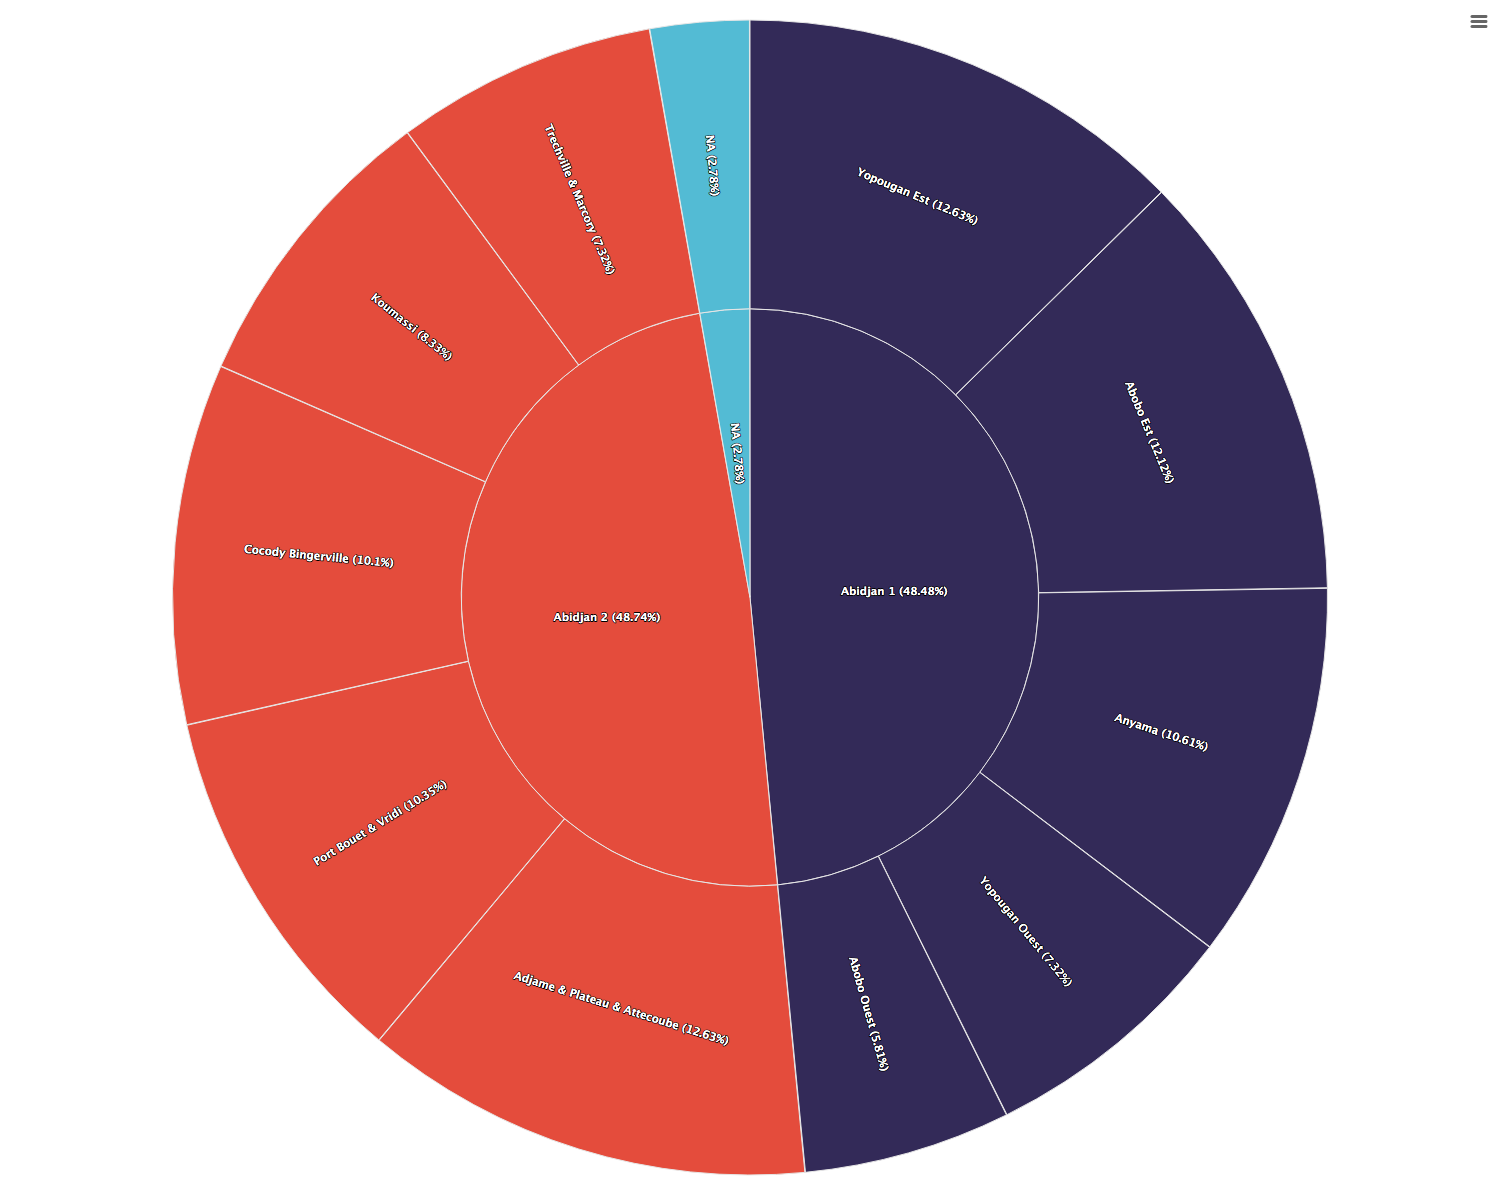
\includegraphics{report_files/figure-latex/unnamed-chunk-9-1.pdf}

\end{document}
